\documentclass[
  bibliography=totoc,     % Literatur im Inhaltsverzeichnis
  captions=tableheading,  % Tabellenüberschriften
  titlepage=firstiscover, % Titelseite ist Deckblatt
]{scrartcl}

% Paket float verbessern
\usepackage{scrhack}

% Warnung, falls nochmal kompiliert werden muss
\usepackage[aux]{rerunfilecheck}

% unverzichtbare Mathe-Befehle
\usepackage{amsmath}
% viele Mathe-Symbole
\usepackage{amssymb}
% Erweiterungen für amsmath
\usepackage{mathtools}

% Fonteinstellungen
\usepackage{fontspec}
% Latin Modern Fonts werden automatisch geladen
% Alternativ:
%\setromanfont{Libertinus Serif}
%\setsansfont{Libertinus Sans}
%\setmonofont{Libertinus Mono}
\recalctypearea % Wenn man andere Schriftarten gesetzt hat,
% sollte man das Seiten-Layout neu berechnen lassen

% deutsche Spracheinstellungen
\usepackage{polyglossia}
\setmainlanguage{german}


\usepackage[
  math-style=ISO,    % ┐
  bold-style=ISO,    % │
  sans-style=italic, % │ ISO-Standard folgen
  nabla=upright,     % │
  partial=upright,   % ┘
  warnings-off={           % ┐
    mathtools-colon,       % │ unnötige Warnungen ausschalten
    mathtools-overbracket, % │
},                       % ┘
]{unicode-math}

% traditionelle Fonts für Mathematik
\setmathfont{Latin Modern Math}
% Alternativ:
%\setmathfont{Libertinus Math}

\setmathfont{XITS Math}[range={scr, bfscr}]
\setmathfont{XITS Math}[range={cal, bfcal}, StylisticSet=1]

% Zahlen und Einheiten
\usepackage[
locale=DE,                   % deutsche Einstellungen
separate-uncertainty=true,   % immer Fehler mit \pm
per-mode=symbol-or-fraction, % / in inline math, fraction in display math
]{siunitx}

% chemische Formeln
\usepackage[
version=4,
math-greek=default, % ┐ mit unicode-math zusammenarbeiten
text-greek=default, % ┘
]{mhchem}

% richtige Anführungszeichen
\usepackage[autostyle]{csquotes}

% schöne Brüche im Text
\usepackage{xfrac}

% Standardplatzierung für Floats einstellen
\usepackage{float}
\floatplacement{figure}{htbp}
\floatplacement{table}{htbp}

% Floats innerhalb einer Section halten
\usepackage[
section, % Floats innerhalb der Section halten
below,   % unterhalb der Section aber auf der selben Seite ist ok
]{placeins}

% Seite drehen für breite Tabellen: landscape Umgebung
\usepackage{pdflscape}

% Captions schöner machen.
\usepackage[
  labelfont=bf,        % Tabelle x: Abbildung y: ist jetzt fett
  font=small,          % Schrift etwas kleiner als Dokument
  width=0.9\textwidth, % maximale Breite einer Caption schmaler
]{caption}
% subfigure, subtable, subref
\usepackage{subcaption}

% Grafiken können eingebunden werden
\usepackage{graphicx}
% größere Variation von Dateinamen möglich
\usepackage{grffile}

% schöne Tabellen
\usepackage{booktabs}

% Verbesserungen am Schriftbild
\usepackage{microtype}

% Literaturverzeichnis
\usepackage[style=alphabetic,]{biblatex}
% Quellendatenbank
\addbibresource{lit.bib}
\addbibresource{programme.bib}

% Hyperlinks im Dokument
\usepackage[
  unicode,        % Unicode in PDF-Attributen erlauben
  pdfusetitle,    % Titel, Autoren und Datum als PDF-Attribute
  pdfcreator={},  % ┐ PDF-Attribute säubern
  pdfproducer={}, % ┘
]{hyperref}
% erweiterte Bookmarks im PDF
\usepackage{bookmark}

% Trennung von Wörtern mit Strichen
\usepackage[shortcuts]{extdash}

\title{US2: Scanverfahren in der Ultraschalltechnik}
\author{
  Simon Schulte
  \texorpdfstring{
    \\
    \href{mailto:simon.schulte@udo.edu}{simon.schulte@udo.edu}
  }{}
  \texorpdfstring{\and}{, }
  Tim Sedlaczek
  \texorpdfstring{
    \\
    \href{mailto:tim.sedlaczek@udo.edu}{tim.sedlaczek@udo.edu}
  }{}
}
\publishers{TU Dortmund – Fakultät Physik}


\date{Durchführung: 20.06.2017\\
      Abgabe: 27.06.2017}

\begin{document}

\maketitle
\thispagestyle{empty}
\tableofcontents
\newpage
\setcounter{page}{1}
\section{Zielsetzung}
\label{sec:zielsetzung}
Ziel des Versuchs ist es, verschiedene Scanverfahren zur
Ultraschallechographie kennenzulernen.
\section{Theorie}
\label{sec:theorie}
Als Ultraschall werden die Schallwellen bezeichnet, die eine Frequenz zwischen
\SI{20}{\kilo\hertz} und \SI{1}{\giga\hertz} haben. Ultraschalluntersuchungen
finden vorallem Verwendung in der Medizin.
Im Gegensatz zu Schall in Flüssigkeiten treten beim Schall durch Festkörper sowohl
Longitudinalwellen als auch Transversalwellen auf. Dabei bezeichnet die Relation
\begin{equation}
  I(x)\,=\,I_0 \cdot e^{\alpha x}
  \label{eqn:intensität}
\end{equation}
die Tatsache, dass die Intensität $I_0$ einer Schallwelle exponentiell mit der
Strecke $x$ abnimmt. Es geht Energie durch Absorption verloren. $\alpha$
bezeichnet dabei den Absorptionskoeffizient der Schallamplitude. \\
\\
Um Ultraschall zu erzeugen wird der piezo-elektrische Effekt genutzt. Dabei
wird ein piezoelektrischer Kristall in ein elektrisches Wechselfeld gegeben.
Dadurch werden Schwingungen im Ultraschallbereich angeregt. Es ist auch möglich
den Piezokristall als Empfänger zu nutzen. Dann regen die Schallwellen den
Kristall an. \\
\\
Abbildung \ref{fig:US22} zeigt das Durchschallungsverfahren. Ein
Ultraschallsender sendet einen kurzzeitigen Schallimpuls aus. Dieser wird am
anderen Ende des Probenstücks mit einem Ultraschallempfänger aufgefangen. Diese
Methode bietet den Vorteil, dass sie zwar zuverlässig Fehlstellen im Material
feststellen kann, aber nicht deren genauen Ort vorhersagen.
\begin{figure}[H]
  \centering
  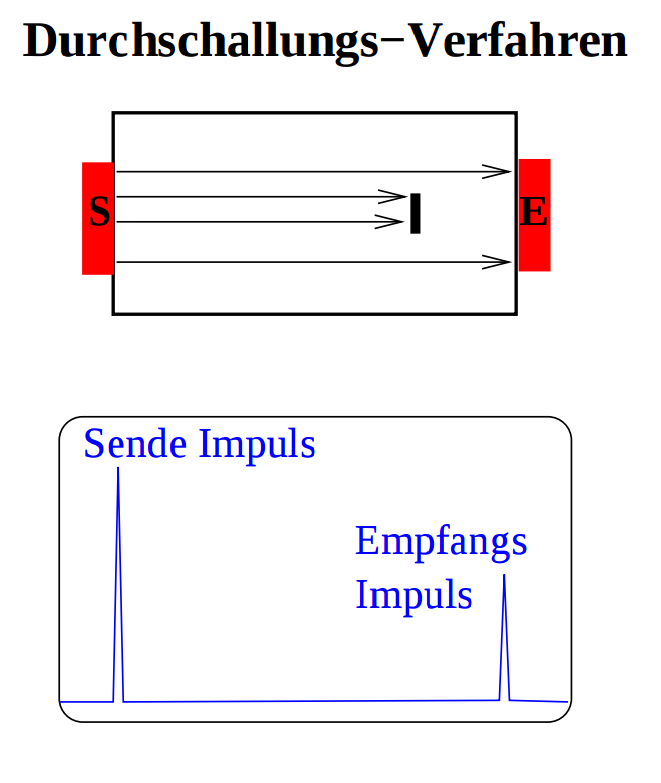
\includegraphics[width=0.5\textwidth]{US22.png}
  \caption{Das Durchschallungsverfahren. \cite{anleitung}}
  \label{fig:US22}
\end{figure}
\noindent
Abbildung \ref{fig:US23} zeigt das Impuls-Echo-Verfahren. Hier wird erneut ein
Schallimpuls von einem Ultraschallsender ausgesendet. Beim
Impuls-Echo-Verfahren wird dieser allerdings an einer Grenzfläche reflektiert
und vom Ultraschallsender wieder aufgenommen. Somit lassen sich auch Aussagen
über die Größe der Fehlstelle machen. Dafür wird die Formel
\begin{equation}
  s\,=\, \frac{1}{2} c t
  \label{eqn:strecke}
\end{equation}
genutzt. Dabei bezeichnet $c$ die Schallgeschwindigkeit in dem jeweiligen
Medium und $t$ die Zeit.
\begin{figure}[H]
  \centering
  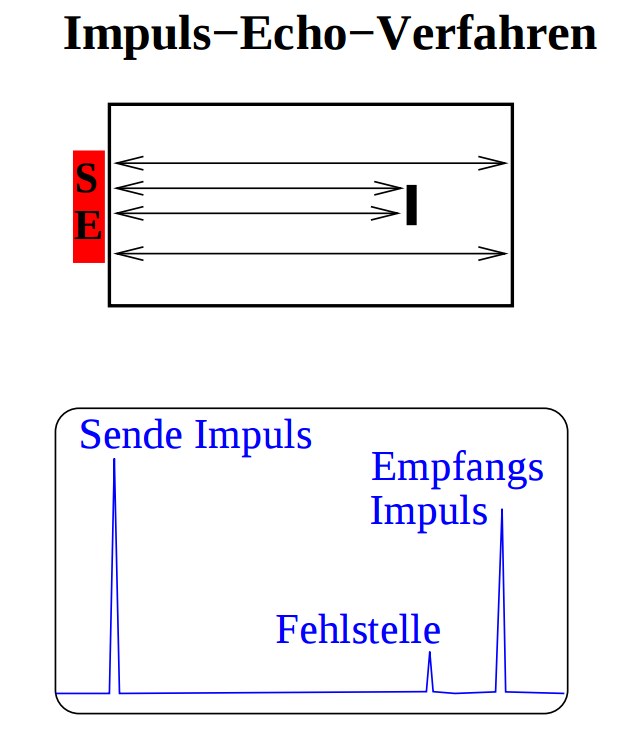
\includegraphics[width=0.5\textwidth]{US23.png}
  \caption{Das Impuls-Echo-Verfahren. \cite{anleitung}}
  \label{fig:US23}
\end{figure}
\noindent
Der Amplituden Scan (A-Scan) stellt die Echoamplituden als Funktion der Zeit
dar. Der A-Scan ist ein eindimensionales Scanverfahren.
Der Brightness Scan (B-Scan) stellt die Echoamplituden in
Helligkeitsabstufungen dar. Der B-Scan ist ein zweidimensionales Scanverfahren.
Dafür muss die Sonde über das zu untersuchende Material bewegt werden.
Der Time-Motion Scan (TM-Scan) kann die Bewegung eines Organs durch eine
schnelle Abtastung aufnehmen.
\section{Versuchsaufbau}
\label{sec:aufbau}
Es werden ein Ultraschallechoskop, eine Ultraschallsonde mit einer Frequenz von
\SI{1}{\mega\hertz} und eine Ultraschallsonde mit einer Frequenz von
\SI{4}{\mega\hertz} verwendet. Diese sind an einen PC angeschlossen, welcher
für die Datenaufnahme und die Datenanalyse verantwortlich ist. Als
Kontaktmittel wird bidestilliertes Wasser genutzt.\\
\\
In diesem Versuch wird ein Acrylblock mit verschiedenen Bohrungen genutzt.
Abbildung \ref{fig:US21} zeigt den Aufbau des verwendeten Acrylblocks.
\begin{figure}[H]
  \centering
  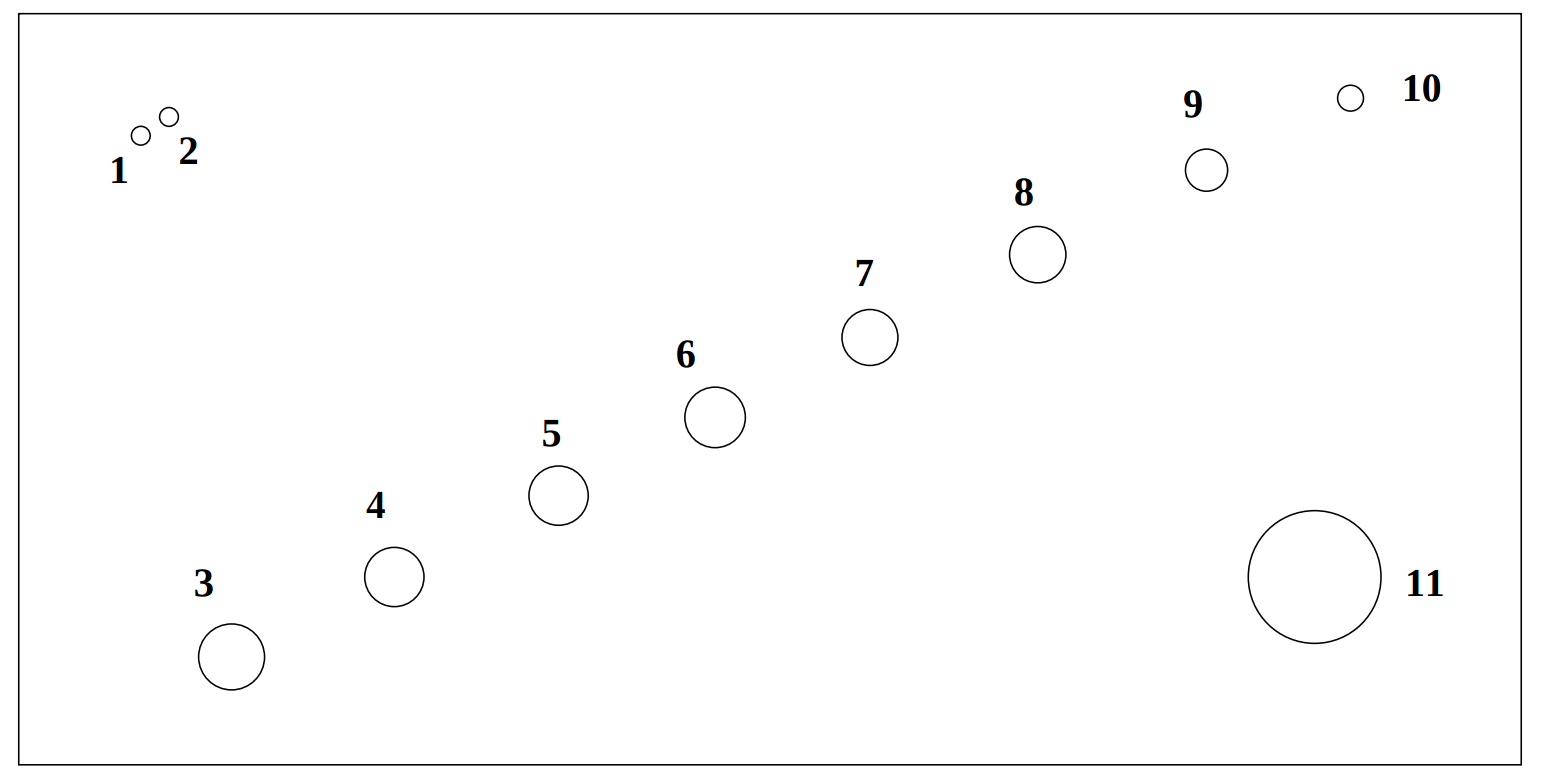
\includegraphics[width=0.7\textwidth]{US21.png}
  \caption{Der Aufbau des Acrylblocks. \cite{anleitung}}
  \label{fig:US21}
\end{figure}
\section{Versuchsdurchführung}
\label{sec:versuchsdurchführung}
Zunächst werden die Abmessungen des verwendeten Acrylblocks mit einer
Schieblehre
bestimmt. Dabei ergeben sich die Werte:
\begin{align*}
  \text{Breite}\,&=\,\SI{15.025}{\centi\meter} \\
  \text{Dicke}\,&=\,\SI{8.04}{\centi\meter} \\
  \text{Tiefe}\,&=\,\SI{4.03}{\centi\meter}.
\end{align*}
Danach wird mit Hilfe des Impuls-Echo-Verfahrens die Lage der Bohrungen im
Acrylblock bestimmt. Dafür wird zunächst etwas destilliertes Wasser auf den
Acrylblock getropft um danach mit einer \SI{1}{\mega\hertz} Sonde den Block zu
untersuchen.
Als Nächstes werden die Tiefen der jeweiligen Störstelle bestimmt. Dafür
werden an verschiedenen Stellen mit Hilfe des A-Scans die Schalllaufzeiten
gemessen. Diese Messung wird nach Umdrehen des Acrylblocks wiederholt. Mit
diesen Werten ist es dann möglich die Größen der Störstellen zu bestimmen.
Als nächstes werden die Bohrungen 1 und 2 genauer betrachtet. Mit einem A-Scan
werden diese beiden Bohrungen nun vermessen, um das Auflösungsvermögen zu
untersuchen.\\
\\
Nun wird der Acrylblock mit dem B-Scan untersucht. Es wird erneut der
Acrylblock mit destilliertem Wasser betröpfelt. Dann wird mit der
\SI{4}{\mega\hertz} Sonde der Block untnersucht. Danach wird die Sonde langsam
und konstant über den Acrylblock geführt, um einen genauen B-Scan zu bekommen.
Danach wird der Block umgedreht und die Messung wiederholt. Als letzten Teil
der Untersuchung des Acrylblocks mit dem B-Scan werden aus den erlangten
Bildern die Abmessungen der Störstellen bestimmt. \\
\\
Als Letztes wird mit Hilfe des TM-Scans ein Herzmodell untersucht. Das
Herzmodell wird dafür zu etwa einem Drittel mit Wasser befüllt und die Sonde so
positioniert, dass sie grade so einen vollständigen Kontakt zur
Wasseroberfläche hat.
Dann wird die Laufzeit des Echos mit einem A-Scan bestimmt. Dann wird eine
Herzfrequenz simuliert. Diese wird mit einem TM-Scan
aufgenommen. Mit den gemessenen Daten lässt sich dann auch das Herzvolumen
bestimmen.\\
\\
Für die Schallgeschwindigkeiten ergeben sich die Werte \cite{olympus} \cite{spektrum}:
\begin{align*}
  v_L\,&=\,\SI{343}{\meter\per\second} \\
  v_W\,&=\,\SI{1450}{\meter\per\second} \\
  v_A\,&=\,\SI{2730}{\meter\per\second}.
\end{align*}
Dabei bezeichnet $v_L$ die Schallgeschwindigkeit in der Luft, $v_W$ die
Schallgeschwindigkeit in destilliertem Wasser und $v_A$ die
Schallgeschwindigkeit in Acryl.
\clearpage
\section{Auswertung}
\label{sec:auswertung}
Zu Beginn werden die Positionen und Größen der Störstellen im Acrylblock
mit einem A-Scan mit der $\SI{1}{\mega\hertz}$-Sonde bestimmt.
Dazu werden die in Tabelle \ref{tab:messwerte1} stehenden Werte für
die Laufzeiten gemessen. Diese werden um $\SI{1.8}{\micro\second}$ korrigiert,
da dies der Dicke des Ausgangssignals entspricht und somit der Dicke der
Schutzschicht. Der Wert wird graphisch aus der Dicke des roten Streifens bei
den B-Scans bestimmt. Beispielhaft sind in Abbildung \ref{fig:plot1} und
Abbildung \ref{fig:plot2} die Verläufe für das sechste und das neunte Loch
dargestellt.
\begin{figure}[H]
  \centering
  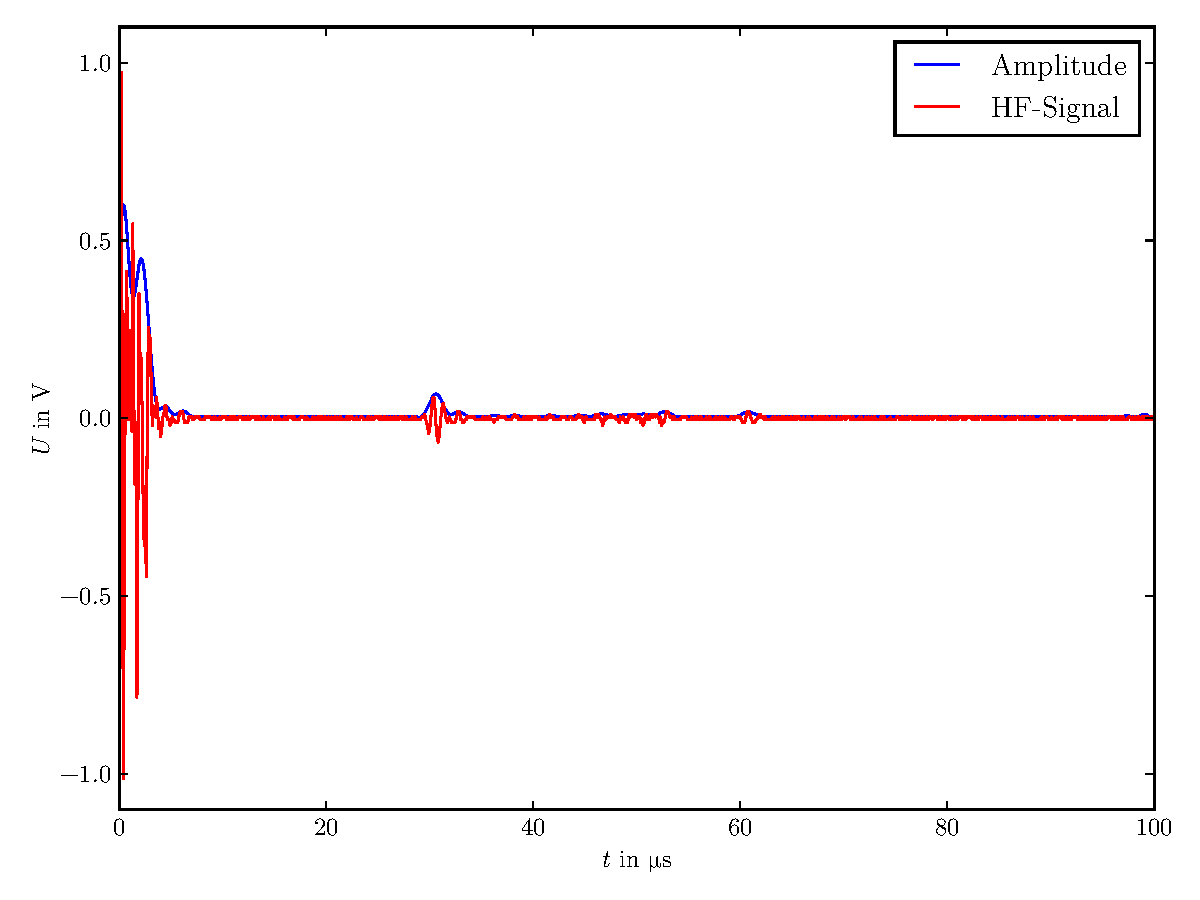
\includegraphics[width=\textwidth]{Plot.pdf}
  \caption{A-Scan Loch Nr.6.}
  \label{fig:plot1}
\end{figure}
\begin{figure}[H]
  \centering
  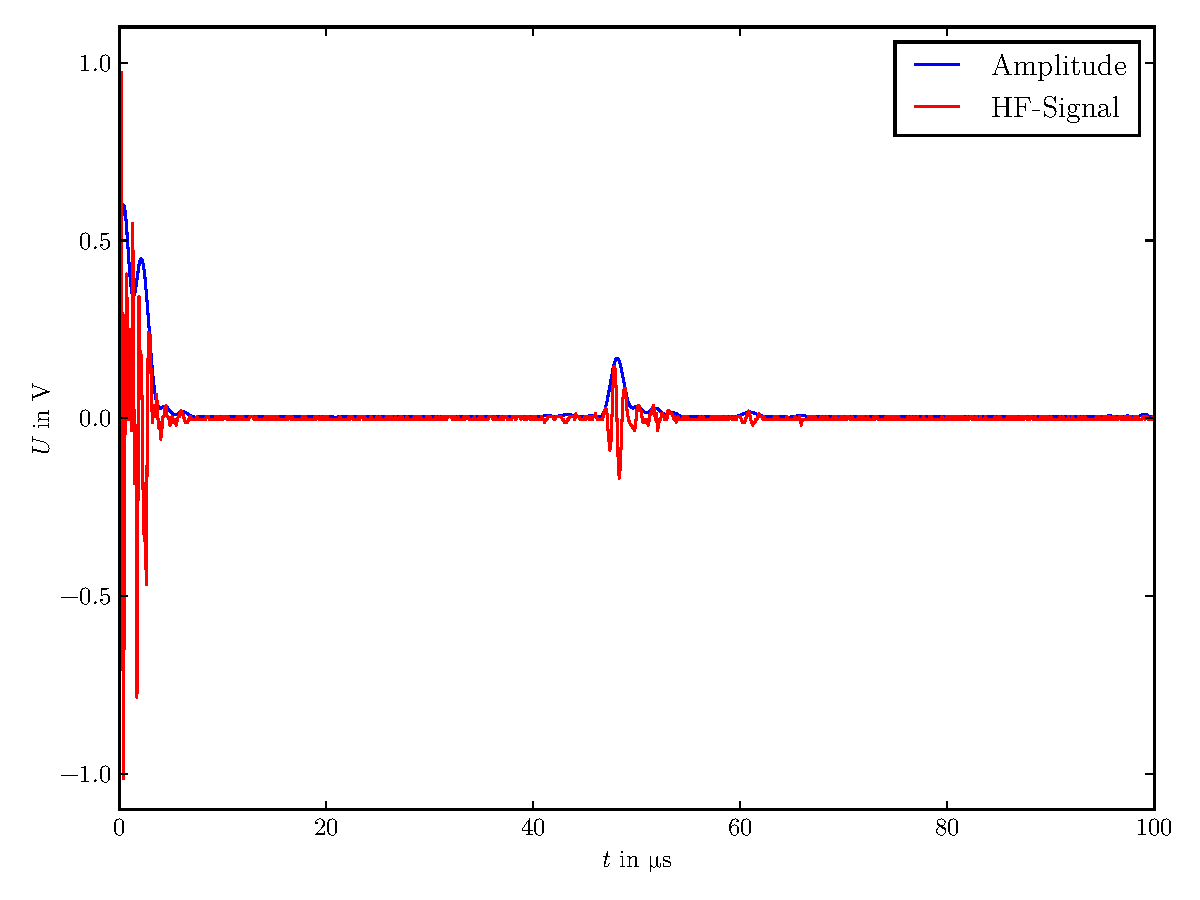
\includegraphics[width=\textwidth]{Plot2.pdf}
  \caption{A-Scan Loch Nr.9.}
  \label{fig:plot2}
\end{figure}
\noindent
Nach Formel \eqref{eqn:strecke}
lässt sich aus den Laufzeiten der Abstand bestimmen.
$c$ beträgt dabei für den Acrylblock
\begin{equation*}
  c = \SI{2730}{\meter\per\second}.
\end{equation*}
Durch Abziehen beider Abstände von der Gesamtdicke des Blocks ergeben sich die
Größen $g$ der Störstellen.
Die daraus resultierenden Positionen und Größen der Störstellen stehen
ebenfalls in Tabelle \ref{tab:messwerte1}.
\begin{table}[H]
  \centering
  \caption{Messwerte und Ergebnisse beim A-Scan.}
  \label{tab:messwerte1}
  \sisetup{table-format=2.1}
  \begin{tabular}{S[table-format=2.1] S S S[table-format=1.2] S[table-format=1.2] S[table-format=2.2]}
    \toprule
    {Loch Nr.} & {$t_1$ in $\si{\micro\second}$} & {$t_2$ in $\si{\micro\second}$} & {$s_1$ in $\si{\centi\meter}$} & {$s_2$ in $\si{\centi\meter}$} & {$g$ in $\si{\centi\meter}$} \\
    & {(ohne Korrektur)} & {(ohne Korrektur)} & {(mit Korrektur)} & {(mit Korrektur)} & \\
    \midrule
     1 & 18.1 & 45.5 & 2.22 & 5.97 & -0.15 \\
     2 & 15.6 & 46.7 & 1.88 & 6.13 &  0.03 \\
     3 & 46.9 & 11.7 & 6.16 & 1.35 &  0.53 \\
     4 & 41.5 & 18.9 & 5.42 & 2.33 &  0.29 \\
     5 & 35.9 & 24.3 & 4.65 & 3.07 &  0.31 \\
     6 & 30.6 & 30.6 & 3.93 & 3.93 &  0.18 \\
     7 & 24.6 & 36.3 & 3.11 & 4.71 &  0.22 \\
     8 & 18.8 & 42.2 & 2.32 & 5.51 &  0.20 \\
     9 & 12.9 & 48.1 & 1.52 & 6.32 &  0.20 \\
    10 &  7.0 & 53.1 & 0.71 & 7.00 &  0.33 \\
    11 & 42.6 & 13.3 & 5.57 & 1.57 &  0.90 \\
    \bottomrule
  \end{tabular}
\end{table}

\noindent
Nun soll das Auflösungsvermögen untersucht werden. Hierzu werden die ersten
beiden Löcher ein zweites mal, mit einer $\SI{4}{\mega\hertz}$-Sonde, vermessen.
Die Messwerte und Ergebnisse stehen in Tabelle \ref{tab:messwerte2}.
\begin{table}
  \centering
  \caption{Messwerte und Ergebnisse beim A-Scan mit $\SI{4}{\mega\hertz}$.}
  \label{tab:messwerte2}
  \sisetup{table-format=2.1}
  \begin{tabular}{S[table-format=1.0] S S[table-format=1.2]}
    \toprule
    {Loch Nr.} & {$t$ in $\si{\micro\second}$ (ohne Korrektur)} & {$s$ in $\si{\centi\meter}$ (mit Korrektur)} \\
    \midrule
     1 & 14.9 & 1.79 \\
     2 & 13.7 & 1.62 \\
    \bottomrule
  \end{tabular}
\end{table}\\

\noindent
Die Positionen und Größen der Störstellen werden nun mit B-Scans erneut gemessen.
Bei der $\SI{1}{\mega\hertz}$-Sonde werden die Abstände graphisch ausgewertet.
Während bei der $\SI{4}{\mega\hertz}$-Sonde die Abstände mit dem Messprogramm
bestimmt werden. Die Ergebnisse stehen in den Tabellen \ref{tab:messwerte3} und
\ref{tab:messwerte4}. Die bei den Scans entstehenden Bilder sind in den
Abbildungen \ref{fig:B-Scan1} bis \ref{fig:B-Scan4} zu sehen.
\begin{table}[H]
  \centering
  \caption{Messwerte und Ergebnisse beim ersten B-Scan.}
  \label{tab:messwerte3}
  \sisetup{table-format=2.1}
  \begin{tabular}{S[table-format=2.1] S S S[table-format=1.2] S[table-format=1.2] S[table-format=2.2]}
    \toprule
    {Loch Nr.} & {$s_1$ in $\si{\centi\meter}$} & {$s_2$ in $\si{\centi\meter}$} & {$g$ in $\si{\centi\meter}$} \\
    \midrule
     1 & 1.7 & 6.0 & 0.3 \\
     9 & 1.3 & 6.0 & 0.3 \\
     2 & 1.7 & 1.2 & 0.7 \\
     3 & 6.1 & 2.0 & 0.7 \\
     4 & 5.3 & 2.9 & 0.5 \\
     5 & 4.6 & 3.8 & 0.3 \\
     6 & 3.9 & 4.6 & 0.4 \\
     7 & 3.0 & 5.4 & 0.4 \\
     8 & 2.2 & 6.2 & 0.5 \\
    10 & 0.5 &  /  &  /  \\
    11 & 5.5 & 1.4 & 1.1 \\
    \bottomrule
  \end{tabular}
\end{table}
\begin{table}[H]
  \centering
  \caption{Messwerte und Ergebnisse beim zweiten B-Scan.}
  \label{tab:messwerte4}
  \sisetup{table-format=2.1}
  \begin{tabular}{S[table-format=2.1] S S S[table-format=1.2] S[table-format=1.2] S[table-format=2.2]}
    \toprule
    {Loch Nr.} & {$t_1$ in $\si{\micro\second}$} & {$t_2$ in $\si{\micro\second}$} & {$s_1$ in $\si{\centi\meter}$} & {$s_2$ in $\si{\centi\meter}$} & {$g$ in $\si{\centi\meter}$} \\
    & {(ohne Korrektur)} & {(ohne Korrektur)} & {(mit Korrektur)} & {(mit Korrektur)} & \\
    \midrule
     1 & 15.8 &   /  & 1.91 &  /   &  /   \\
     2 & 14.5 &   /  & 1.73 &  /   &  /   \\
     3 & 46.3 & 11.4 & 6.07 & 1.31 & 0.66 \\
     4 & 40.9 & 17.5 & 5.34 & 2.14 & 0.56 \\
     5 & 35.3 & 23.6 & 4.57 & 2.98 & 0.49 \\
     6 & 29.9 & 29.7 & 3.84 & 3.81 & 0.40 \\
     7 & 23.9 & 35.6 & 3.02 & 4.61 & 0.41 \\
     8 & 18.3 & 41.5 & 2.25 & 5.42 & 0.37 \\
     9 & 12.6 & 47.4 & 1.47 & 6.22 & 0.34 \\
    10 &  7.0 &   /  & 0.71 &  /   &  /   \\
    11 & 42.2 & 12.7 & 5.51 & 1.49 & 1.04 \\
    \bottomrule
  \end{tabular}
\end{table}
\begin{figure}[H]
  \centering
  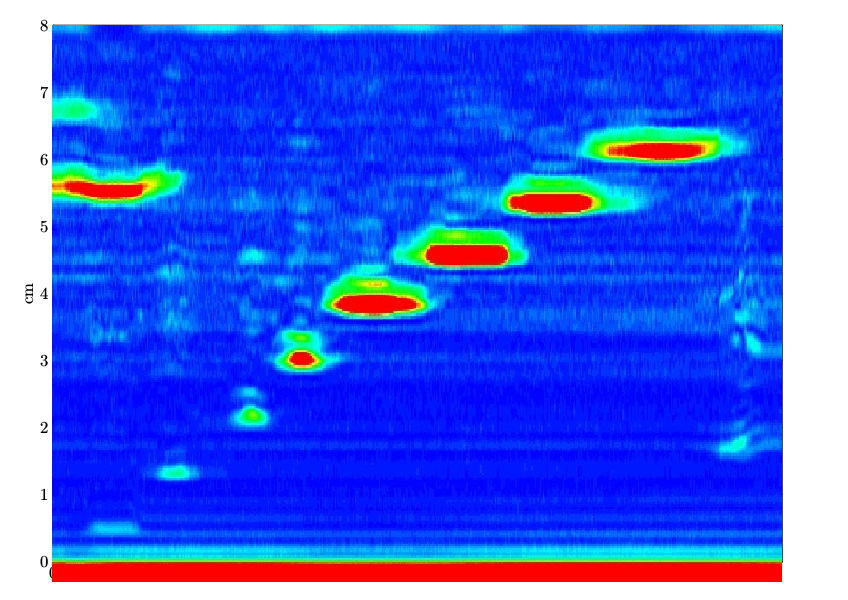
\includegraphics[width=0.88\textwidth]{B-Scan1Mhz1.png}
  \caption{B-Scan mit $\SI{1}{\mega\hertz}$.}
  \label{fig:B-Scan1}
\end{figure}
\begin{figure}[H]
  \centering
  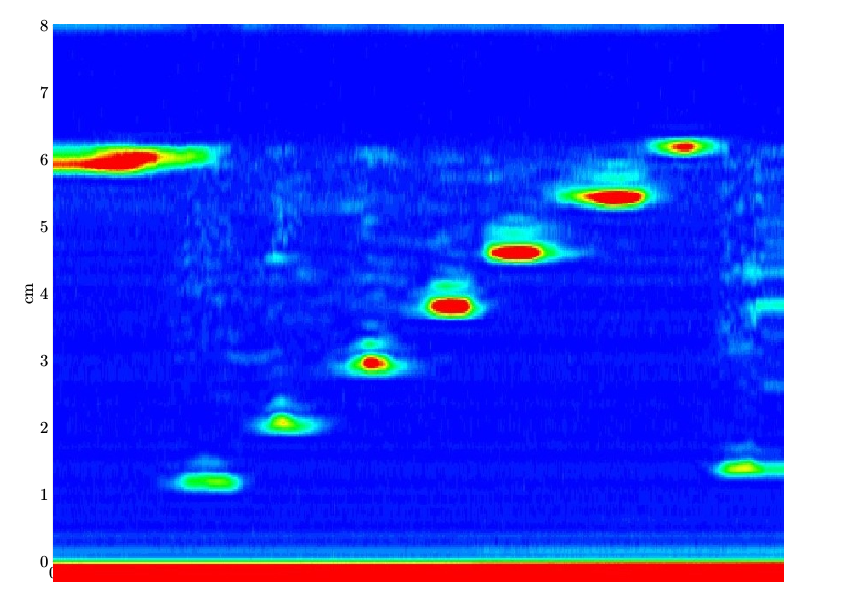
\includegraphics[width=0.88\textwidth]{B-Scan1Mhz2.png}
  \caption{B-Scan mit $\SI{1}{\mega\hertz}$ nach umdrehen des Blocks.}
  \label{fig:B-Scan2}
\end{figure}
\begin{figure}[H]
  \centering
  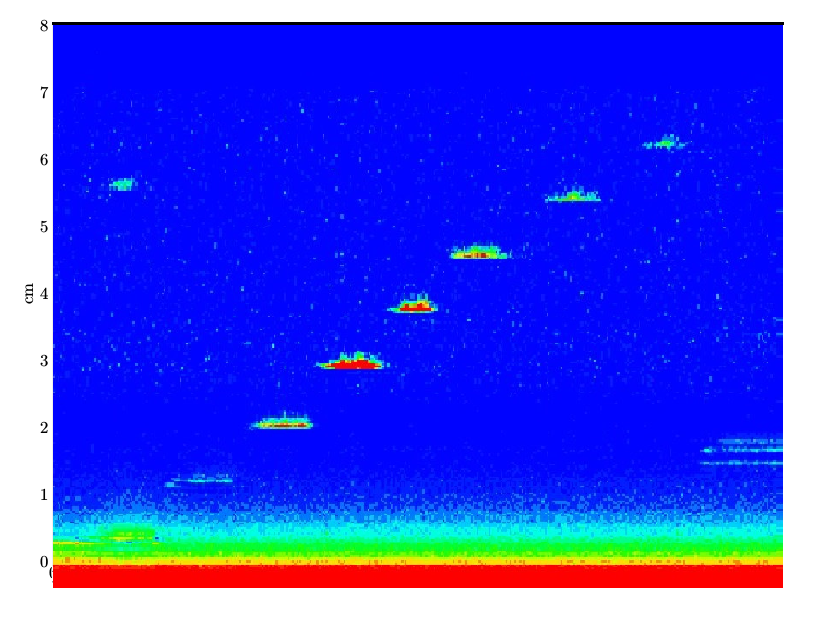
\includegraphics[width=0.83\textwidth]{B-Scan4MHz1.png}
  \caption{B-Scan mit $\SI{4}{\mega\hertz}$.}
  \label{fig:B-Scan3}
\end{figure}
\begin{figure}[H]
  \centering
  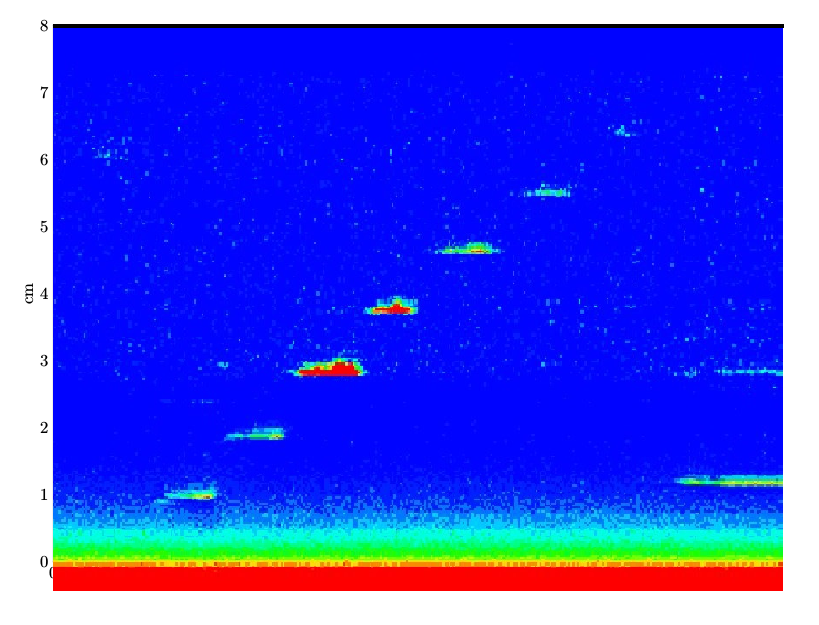
\includegraphics[width=0.83\textwidth]{B-Scan4MHz2.png}
  \caption{B-Scan mit $\SI{4}{\mega\hertz}$ nach umdrehen des Blocks.}
  \label{fig:B-Scan4}
\end{figure}

\noindent
Schließlich wird noch das Herzvolumen eines Herzmodels bestimmt.
Dazu wird die Frequenz bestimmt mit der das Herz aufgepumpt wird und die
durchschnittliche maximale Höhe der Membrane.
Aus den Abständen der Maxima ergibt sich eine Frequenz von $\SI{2}{\hertz}$.
Für die Ersten 11 Maxima von rechts werden die Auslenkungen der Membrane bestimmt.
Die Ergebnisse davon stehen in Tabelle \ref{tab:messwerte5} und das entsprechende
Bild ist in Abbildung \ref{fig:TM} zu sehen.
\begin{table}
  \centering
  \caption{Messwerte und Ergebnisse beim ersten B-Scan.}
  \label{tab:messwerte5}
  \sisetup{table-format=2.1}
  \begin{tabular}{S[table-format=2.1] S S S[table-format=1.2] S[table-format=1.2] S[table-format=2.2]}
    \toprule
    {Maximum Nr.} & {$h$ in $\si{\centi\meter}$} \\
    \midrule
     1 & 2.23 \\
     9 & 2.44 \\
     2 & 2.34 \\
     3 & 2.44 \\
     4 & 2.34 \\
     5 & 2.28 \\
     6 & 2.39 \\
     7 & 2.54 \\
     8 & 2.28 \\
    10 & 2.28 \\
    11 & 2.28 \\
    \bottomrule
  \end{tabular}
\end{table}\\
\begin{figure}[H]
  \centering
  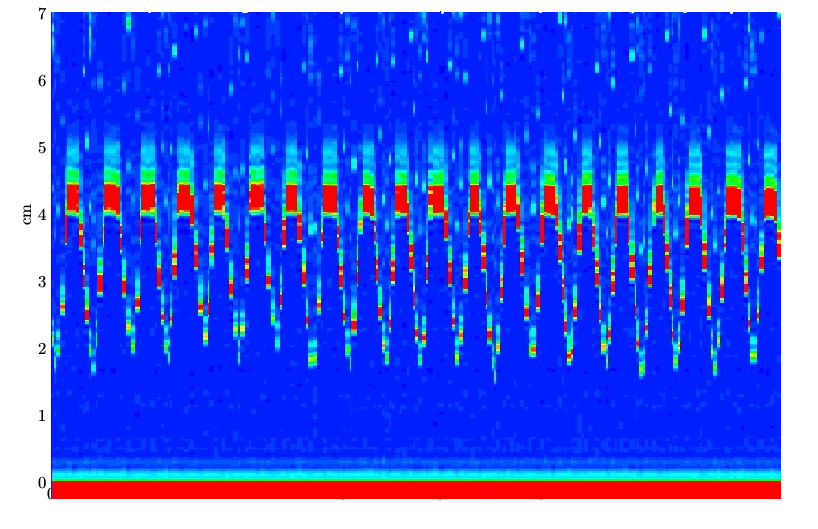
\includegraphics[width=0.93\textwidth]{TM-Scan.png}
  \caption{TM-Scan des Herzmodels.}
  \label{fig:TM}
\end{figure}
\noindent
Die Höhen werden zu
\begin{equation*}
  h = \SI{2.35(3)}{\centi\meter}
\end{equation*}
gemittelt.

\noindent
Näherungsweise wird für die Form der Membrane ein Rotationsparaboloid angenommen.
Dessen Volumen berechnet sich nach
\begin{equation}
  V = \frac{\pi}{2} r^2 \cdot h.
  \label{eqn:parabol}
\end{equation}
\noindent
Dabei ist $r = \SI{2.465}{\centi\meter}$.
Somit ergibt sich mit der zuvor bestimmten Höhe ein enddiastolisches Volumen von
\begin{equation*}
  V = \SI{22.42(27)}{\cubic\centi\meter}.
\end{equation*}
Durch multiplikation mit der Frequenz folgt das Herzvolumen
\begin{equation*}
  HZV = \SI{44.8(5)}{\cubic\centi\meter\per\per\second}.
\end{equation*}
\section{Diskussion}
\label{sec:diskussion}
In Tabelle \ref{tab:ergebnissevers} stehen die Ergebnisse vom A- und vom B-Scan.
\begin{table}[H]
  \centering
  \caption{Ergebnisse A-/B-Scan.}
  \label{tab:ergebnissevers}
  \sisetup{table-format=1.2}
  \begin{tabular}{S[table-format=2.0] S[table-format=2.2] S[table-format=1.1] S}
    \toprule
    & {A-Scan $\SI{1}{\mega\hertz}$} & {B-Scan $\SI{1}{\mega\hertz}$} & {B-Scan $\SI{4}{\mega\hertz}$} \\
    {Loch Nr.} & {$g$ in $\si{\centi\meter}$} & {$g$ in $\si{\centi\meter}$} & {$g$ in $\si{\centi\meter}$} \\
    \midrule
     1 & -0.15 & 0.3 &  /   \\
     2 &  0.03 & 0.3 &  /   \\
     3 &  0.53 & 0.7 & 0.66 \\
     4 &  0.29 & 0.7 & 0.56 \\
     5 &  0.31 & 0.5 & 0.49 \\
     6 &  0.18 & 0.3 & 0.40 \\
     7 &  0.22 & 0.4 & 0.41 \\
     8 &  0.20 & 0.4 & 0.37 \\
     9 &  0.20 & 0.5 & 0.34 \\
    10 &  0.33 &  /  &  /   \\
    11 &  0.90 & 1.1 & 1.04 \\
    \bottomrule
  \end{tabular}
\end{table}
\noindent
Die Größen liegen bei allen drei Messungen im gleichen Bereich.
jedoch weicht der A-Scan etwas stärker von den B-Scans ab. Ein Loch hat demnach
sogar eine negative Größe. Das liegt wahrscheinlich daran, dass die Korrektur
aus dem B-Scan bestimmt wurde und dadurch nicht ganz zu dem A-Scan passt.
Insgesamt sind einige kleine Schwankungen zu sehen, was an Ablesefehlern liegen
könnte, da sich die entsprechenden Stellen, wie in den Abbildungen zu sehen
ist, über einen größeren Bereich strecken. Diese Bereiche werden mit
zunehmender Frequenz des Ultraschalls kleiner und schärfer. Die Größen, die
bei $\SI{4}{\mega\hertz}$ gemessen wurden wirken am sinnvollsten.
Manche Größen sind bei den B-Scans nicht messbar, da die entsprechenden
Störstellen im Schattenbereich einer anderen Störstelle liegen oder wegen zu
großer Distanzen nicht mehr von der Sonde erfasst wurden.

\noindent
Zu dem Auflösungsvermögen gibt es die in Tabelle \ref{tab:ergebnissevers2}
stehenden Ergebnisse.
\begin{table}[H]
  \centering
  \caption{Ergebnisse bei der Messung des Auflösungsvermögens.}
  \label{tab:ergebnissevers2}
  \sisetup{table-format=2.1}
  \begin{tabular}{S[table-format=1.0] S S[table-format=1.2]}
    \toprule
    & {$\SI{1}{\mega\hertz}$} & {$\SI{4}{\mega\hertz}$} \\
    {Loch Nr.} & {$s$ in $\si{\centi\meter}$} & {$s$ in $\si{\centi\meter}$} \\
    \midrule
     1 & 2.22 & 1.79 \\
     2 & 1.88 & 1.62 \\
    \bottomrule
  \end{tabular}
\end{table}
\noindent
Die Werte unterscheiden sich ebenfalls um $\SI{0.2}{\centi\meter}$ bis $\SI{0.5}{\centi\meter}$.
Bei der Messung mit der $\SI{1}{\mega\hertz}$-Sonde waren die beiden Löcher jedoch
kaum zu unterscheiden. Erst mit der $\SI{4}{\mega\hertz}$-Sonde waren die beiden
einzelnen Störstellen gut zu unterscheiden.

\noindent
Mit der Messung des Herzvolumens ist gut zu sehen, dass die Ultraschalltechnik
trotz gewisser Ungenauigkeiten bzgl. exakter Abstände gut für medizinische
zwecke geeignet ist. Die Ungenauigkeiten lassen sich sogar mit entsprechend
hohen Frequenzen minimieren.
\clearpage
\nocite{*}
\printbibliography
\end{document}
